\chapter{GeV-scale non-accelerator physics program}
\label{ch:nonaccel}


%%%%%%%%%%%%%%%%%%%%%%%%%%%%%%%%%%%%%%%%%%%%%%%%%%%%%%%%%%%%%%%%
\section{Nucleon decay}
\label{sec:nonaccel-ndk}

Unification of three of the fundamental forces in the universe, the strong, 
electromagnetic and weak interactions, is a central paradigm for the current 
world-wide program in particle physics. Grand Unified Theories (GUTs), aiming 
at extending the standard model of particle physics to include a unified force 
at very high energies  (above $10^{15}$ GeV), predict a number of observable 
effects at low energies, such as nucleon 
decay \cite{Pati:1973rp,Georgi:1974sy,Dimopoulos:1981dw,Langacker:1980js,deBoer:1994dg,Nath:2006ut}. 
Several experiments have been searching for signatures of nucleon decay, with the best limits 
for most decay modes set by the Super-Kamiokande experiment \cite{Nishino:2012bnw}, 
which features the largest sensitive mass to date. 


\subsection{Predictions from Grand Unified Theories and current experimental status}
\label{subsec:nonaccel-ndk-status}

\todo{need theorist input?}
\begin{description}
\item[Predictions and experimental status:] Plot or table with partial lifetime predictions for dominant NDK channels in selected GUT theories, together with current limits for each channel.
\end{description}
\todo{Need pretty limit plot}

\subsection{Experimental signatures for nucleon decay searches in DUNE}
\label{subsec:nonaccel-ndk-dune}

The DUNE far detector, as the largest active volume of argon, 
will be highly sensitive to a number of possible nucleon decay modes, 
in many cases complementing the capabilities of large water detectors.  
In particular, the \lartpc technology is expected to be well-suited for observing 
nucleon decays into charged kaons, which can be identified with redundancy 
from their distinctive $dE/dx$ signature as well as by their decays.
%have advantages over water detectors for observing nucleon decays into charged kaons, which are below Cherenkov threshold in water. These modes are favored by SUSY models, and the tests of these models are within reach of multi-kiloton \lartpc{}s such as DUNE. 
A particularly interesting mode for the proton decay search with DUNE is 
$p\to K^+ \bar{\nu}$, which is expected to have a lifetime of the order of 
$>10^{33}$ years in SUSY models. This decay can be tagged in a \lartpc if a 
single kaon within a proper energy/momentum range can be reconstructed with 
its point of origin lying within the fiducial volume. 
Background events initiated by cosmic-ray muons can be controlled  by requiring 
no activity close to the edges of the TPCs and by stringent single kaon identification 
within the energy range of interest. 
Atmospheric neutrino-induced background with real kaon production will either have an 
associated strange baryon (for reactions with $\Delta S = 0$) whose decay can be 
reconstructed, or an identifiable charged lepton (for reactions with $\Delta S = 1$). 
Atmospheric neutrino-induced background may also arise from misidentification of protons 
from abundant quasielastic interactions.  Work is ongoing (see below) to understand 
in detail how to fully exploit the capabilities of the DUNE \lartpc FD modules to suppress the above 
backgrounds while maintaining the high acceptance necessary for discovery-level sensitivity.
Similarly, the DUNE FD is expected to have good sensitivity to other compelling 
nucleon decay modes, 
such as $n\to K^+ e$, $p\to l^+ K^0$, and $p\to \pi^0 e^+$, which are also under study. \todo{This paragraph needs updated.}

Monte Carlo studies of the $p\to K^+ \bar{\nu}$ signal and corresponding atmospheric neutrino backgrounds have been carried out with the DUNE multi-purpose full event reconstruction software.  They reveal that the main challenge in identifying proton decay candidates is due to backgrounds arising from the mis-reconstruction of protons as positive kaons. This happens when a charged current (CC) neutrino interaction produces a muon and a recoiling proton and the primary vertex for neutrino interaction is mis-labelled as a secondary vertex where the kaon decays.  Complicating the ability to reject pathological events of this type is the presence of final state interactions (FSI) in proton decay, which can shift the spectrum of kaons towards low energies, with possible concurrent emission of nucleons, which together weaken the otherwise distinct energy and $dE/dx$ signature of the kaon. Ongoing work to reject these backgrounds without loss of acceptance includes implementation of convolutional neural networks, as well as efforts to understand the uncertainty associated with the intra-nuclear cascade model. 

\subsubsection{Final State Interactions}
\label{sec:final-state-interactions}

In a proton decay via $p\rightarrow K^{+} \bar{\nu}$, the charged kaon may interact on its way out of the nucleus, and these final state interactions significantly modify the observable distributions in the detector. 

The simulation of nucleon decay events is performed using the GENIE Neutrino Monte Carlo Generator (GENIE) \cite{genie} v.2.12.10 . A total of 68 single-nucleon exclusive decay channels listed in the 2016 update of the PDG book is available in GENIE. The list includes two-, three- and five-body decays. 
%The numbering in the decay modes follows the PDG convention.  
The primary decay is simulated using a phase-space-decay generator. 
%For bound nucleons, the nuclear environment is simulated as in neutrino scattering. 
%The nucleon is assigned a Fermi momentum and removal energy and it is off the mass shell.  
The relativistic Fermi gas (RFG) nuclear model is used with a Bodek-Ritchie  tail to incorporate short range nucleon-nucleon correlations (add citation).
%\cite{BRtail}. 
For $^{40}$Ar the Fermi momentum has a default value of 242.0 MeV/c with binding energy = 27.0 MeV. 
%Fig \ref{fig:pdcy_m} shows the momentum distribution for a bound proton in $^{40}$Ar. 
If a bound nucleon decays the remaining nucleus can be in an excited state and will typically de-excite by emitting nuclear fission fragments, nucleons, and photons. At present de-excitation photon emission is simulated only for oxygen.  However, measurements of argon de-excitation gamma in LArTPC detectors have been reported by the ArgoNeuT collaboration (cite new paper),
%\cite{Argoneut}, 
where energy depositions and positions of these depositions have been compared to those from simulations of neutrino-argon interactions using the FLUKA Monte Carlo generator. 
%\cite{geniemanual}. 
The propagation of the decay products is simulated using an intra-nuclear cascade Monte Carlo (MC). The probability $\lambda$ that a particle will undergo an interaction is governed by the free cross section $\sigma$ and the density of nucleons $\rho$,
\begin{equation}
\lambda(E,r)= \frac{1}{\sigma \rho(r)}.
\end{equation}
The type of interaction is then chosen according to the cross sections for various reactions for free nucleons, sometimes modified for nuclear medium effects, relative to the total cross section. Charged kaons can undergo various scattering process in the nucleus such as elastic scattering, charge exchange, absorption (only $K^{-}$; $K^{+}$ absorption is forbidden due to baryon number conservation in the nucleus), and $K^{+}$ production via $\pi^{+}+N$ reaction via strong processes such as $\pi^{+}n \rightarrow K^{+} \Lambda$.

In this analysis, the $hA2015$ model in GENIE is used as the default model for FSI.  $hA2015$ is an empirical, data-driven method which does not model the cascade of hadronic interactions step by step, but instead uses one effective interaction where hadron+nucleus data is used to determine the final state.  \todo{Is this description right? Citation for hA2015}
For kaons $K^{+}+C$ data 
%\cite{K+C1,K+C2} 
is used when available. $hA2015$ only considers elastic scattering, and therefore a kaon is never added to or removed from the final state. Fig. \ref{fig:K-wFSI-hA2015} shows the kaon kinetic energy before and after FSI. Due to FSI the kaon spectrum becomes softer on average. 31.5$\%$ of the kaons undergo elastic scattering resulting in events with very low kinetic energy, with $25\%$ of kaons having a kinetic energy of $\le$50 MeV. When the kaon undergoes elastic scattering, a nucleon can be knocked out of the nucleus. $26.7\%$ of decays via this channel have one neutron coming from FSI, $15.3\%$ have at least one proton, and $10.3\%$ have two protons coming from FSI. These secondary nucleons have a detrimental effect on the reconstruction and selection of $K^{+}$.\todo{add citations}

\begin{dunefigure}[Kaon kinetic energy before and after FSI]{fig:K-wFSI-hA2015}{Kinetic energy of kaons in simulated proton decay events, $p\rightarrow K^{+} \bar{\nu}$.  The kinetic energy distribution is shown before and after final state interactions in the argon nucleus.}
\includegraphics[width=0.8\textwidth]{K-wFSI-hA2015.pdf}
\end{dunefigure}

%To compare the size of FSI effects in argon with the effects in previous searches in a water Cherenkov detector,
%\cite{sk2}
%only 0.14$\%$ of kaons go under charge-exchange \todo{in water? in oxygen?} where $hN$ predicts $14.8\%$ in argon.  For a carbon nucleus $hA$ predicts  $13\%$ of kaons undergo elastic scattering before exiting the nucleus whereas in argon $31.5\%$ do. \todo{Do we have first number from hA?}

\subsubsection{Event reconstruction}
\label{sec:event-reconstruction}

\todo{Refer to reconstruction chapter}

Track reconstruction efficiency for a charged particle $x^{\pm}$ is defined as 
\begin{equation}
\epsilon_{x^{\pm}} = \frac{\mbox{$x^{\pm}$ particles with a reconstructed track}}{\mbox{events with $x^{\pm}$ particle }}.
\end{equation}
The denominator includes events in which an $x^{\pm}$ particle was created and has deposited energy within any of the TPCs.  The numerator includes events in which an $x^{\pm}$ particle was created and has deposited energy within any of the TPCs and a reconstructed track can be associated to the $x^{\pm}$ particle based on the number of hits generated by that particle along the track. This efficiency can be calculated as a function of true kinetic energy and true track length.

\begin{dunefigure}[Tracking efficiency of kaons in $p\rightarrow K^{+} \bar{\nu}$]{fig:k-trk-eff}{Tracking efficiency for kaons in simulated proton decay events, $p\rightarrow K^{+} \bar{\nu}$, as a function of kaon kinetic energy (left) and true path length (right).}
\includegraphics[width=0.4\textwidth]{k-trk-eff-KE.pdf}
\includegraphics[width=0.4\textwidth]{k-trk-eff-length.pdf}
\end{dunefigure}

Fig. \ref{fig:k-trk-eff} shows tracking efficiencies for $K^{+}$  from proton decay. The integrated tracking efficiency for kaons is 58.0$\%$, and based on Fig.\ref{fig:k-trk-eff} the tracking threshold is approximately $\sim$30-40 MeV of kinetic energy. This translates to $\sim$4.0 cm in length. It is import to mention that 22.5$\%$ of kaons have kinetic energy$<$40 MeV which is below the tracking threshold. Another feature of the tracking efficiency is that there is a plateau of $80\%$ above 80 MeV of kinetic energy; the 20$\%$ inefficiency is due to prompt decays. Kaon scattering in LAr is a small effect (less than 0.1$\%$ of kaons re-scatter in the LAr), but charge exchange in LAr occurs is a bigger effect with 1.2$\%$ of kaons experiencing charge exchange. Both of these processes are included in the simulation.  Overall the biggest loss in tracking efficiency is due to kaons carrying only a few MeV of kinetic energy due to scattering inside the nucleus as described in Section~\ref{sec:final-state-interactions}

Another metric useful to evaluate track performance is the completeness and purity of the track. Completeness is defined as
 \begin{equation}
Completeness = \sum_{i}^{\mbox{track hits}}\frac{\mbox{(hit energy on track from a charged particle)}_{i}}{\mbox{total hit energy from a charged particle}},
\end{equation}
where completeness equal to one means all the hits associated with a charged particle were reconstructed as a single track. 
Fig. \ref{fig:k_complet_purity} shows the track completeness for $K^{+}$ from proton decay events. The peak at 0.667 is due to the three-plane design of the TPC.  If a particle travels parallel to a wire plane it is very likely that the reconstruction algorithm cannot match the two-dimensional clusters of hits in all three views.  This results in a track with a completeness of 2/3 (0.667), with 1/3 of the hits not associated to the track.  This feature has an impact on particle identification since it causes misreconstruction of the decay point, where the $dE/dx$ information is most useful.

Track purity is the estimated level of hit contamination from another particle, defined as
\begin{equation}
Purity = \sum_{i}^{\mbox{track hits}}\frac{\mbox{(hit energy on track from a charged particle)}_{i}}{\mbox{total hit energy on the track}},
\end{equation}
Fig \ref{fig:k_complet_purity} shows the track purity for $K^{+}$ from proton decay events. The average purity for a kaon track is $\sim0.94$. Of the 16$\%$ of the kaon tracks with lower purity than average, in most cases this is due to a proton and kaon overlapping in a single track. This will also impact the performance of the particle identification since the information on $dE/dx$ is misleading due to overlap of a different particle. 

\begin{dunefigure}[Completeness and purity of kaon tracks in $p\rightarrow K^{+} \bar{\nu}$]{fig:k_complet_purity}{Completeness (left) and purity (right) for kaon tracks in simulated proton decay events, $p\rightarrow K^{+} \bar{\nu}$.}
\includegraphics[width=0.4\textwidth]{k_complet.pdf}
\includegraphics[width=0.4\textwidth]{k_purity.pdf}
\end{dunefigure}

The branching fraction for leptonic decay of charged kaons, $K\rightarrow \mu \nu_{\mu}$, is approximately 64$\%$. The remaining decay modes are semileptonic or hadronic and include charged and neutral pions. The leptonic decay offers a distinguishable topology with a heavy ionizing particle followed by a minimum ionizing particle. In addition, given the kinematics of a proton decay event, 95.0$\%$ of the kaons decay at rest. Using two-body kinematics, the momentum of the muon is approximately 237 MeV/c. The reconstructed momentum of the muon offers a powerful discriminating variable to separate signal from background events. 
%Fig \ref{fig:mu_complet_purity} shows track completeness and purity for $\mu^{+}$ from kaon decay. Track purity for muons has a wider distribution this is caused by EM contribution coming  from delta rays and/or Bremsstrahlung photons. Momentum and residual for muons are shown in Fig. \ref{fig:mu_p}. As expected from the kaon decay at rest most the muon tracks have a reconstructed momentum of 237 MeV/c, there is a long tail in both momentum and residual distributios, this is due to muon broken tracks that have been split by delta rays.

Charged particles lose energy through ionization and scintillation when traversing the LAr, and this energy loss provides valuable information on particle energy and species. To identify a given particle the hits associated with a reconstructed track are used.
%For each hit the ADC counts are converted to charge $Q_{rec}$. To account for the charge loss along the drift due to impurities, a correction is applied to $Q_{rec}$, $Q = Q_{rec}/e^{-t/\tau}$,  where $t$ is the electron drift time for the hit and $\tau$ is the electron lifetime. The charge $Q$ is divided by the track pitch $dx$. Finally, to account for charge loss due to recombination, a second correction is applied to convert $dQ/dx$ to $dE/dx$ based on the Birks's model \cite{PIDAref1}. 
The total energy deposition from the track is obtained by summing the $dE/dx$ for all the reconstructed hits. If the charged particle stops in the LArTPC active volume, $dE/dx$ as a function of the residual range ($R$), the path length to the end point of the track, is used for particle identification as
\begin{equation}
<PIDA >= \left(\frac{dE}{dx}\right)_{i}R^{0.42}_{i}, 
\end{equation}
which is defined to be the median over all track points where the residual range $R$ is less than 30 cm. This procedure can be done for each plane. 

\begin{dunefigure}[Particle identification for $p\rightarrow K^{+} \bar{\nu}$]{fig:PIDA}{Particle identification (PIDA) for particles in simulated proton decay events, $p\rightarrow K^{+} \bar{\nu}$.}
\includegraphics[width=0.8\textwidth]{PIDA.pdf}
\end{dunefigure}

Fig \ref{fig:PIDA} shows the $<$PIDA$>$ performance for kaons (from proton decay), muons (from kaon decay) and protons produced by atmospheric neutrino interactions. The tail with lower values in each distribution is due to cases where the decay/stopping point was missed by the track reconstruction. The tail with higher values is caused when a second particle overlaps at the decay/stopping point causing higher values of $dE/dx$ resulting in higher values of PIDA. In addition ionization fluctuations smear out this distributions.

\subsubsection{Backgrounds}
\label{sec:ndkbkgd}

The main background for proton decay searches is interactions of  atmospheric neutrinos. In this analysis, the Bartol flux is used. \todo{Add citation.  Do we need details?}
%\cite{Bartolref} at Soudan location is used, the Bartol flux is a MC calculation of the atmospheric neutrino fluxes, the calculations starts with simulations of the interactions of the primary cosmic rays with the atmosphere. The earth is assumed to be a sphere and primaries are generated with random positions and angles. The effect of the geomagnetic field on the interacting cosmic rays is included by applying the cutoff using the back-tracing technique \cite{Bartolref} . 
%Fig \ref{fig:atmo_flux} shows the atmospheric flux prediction for different neutrino species.
Neutrino interactions in argon are simulated with GENIE. To estimate the event rate we integrate the  flux times cross section. Table \ref{tab:rate} shows the event rate for different neutrino species for an exposure of 10~kton-years.

\begin{dunetable}
[Expected rate of neutrino interactions in $^{40}$Ar for 10~kton-year exposure.]
{cccc}
{tab:rate}
{Expected rate of neutrino interactions in $^{40}$Ar for 10~kton-year exposure.}
  ~10kton-year~   &~CC~&~NC~&~Total \\
$\nu_{\mu}$ & 1038 & 398 &1436 \\
$\bar{\nu}_{\mu}$ &280 & 169 & 449 \\
$\nu_{e}$ & 597 &  206 &83 \\
$\bar{\nu}_{e}$ & 126 & 72 & 198 \\
Total & 2014 & 845 & 2886 \\
\end{dunetable}

\subsubsection{Event Classification}

The proton decay $p\rightarrow K^{+} \bar{\nu}$ signal and atmospheric neutrino background events are processed through the same reconstruction chain and subject to the same selection criteria. A pre-selection is applied to remove obvious background. The pre-selection cuts require at least two tracks in the event and that the longest track is not greater than 100 cm in length. The efficiency for the pre-selection cuts is 50$\%$ for signal and 17.5$\%$ for background.
 
Multivariate classification methods based on machine learning techniques have become a fundamental ingredient to most analyses in HEP. 
%Decision trees are well known classifiers, and differ from a cut-based analysis that selects only in one dimension of the phase space, a decision tree is able to split the phase space into a large number of dimensions (variables). A potential issue with a decision tree is its instability with respect to statistical fluctuations in the training sample from which the tree structure is derived. For example, if two input variables exhibit similar separation power, a fluctuation in the training sample may cause the tree growing algorithm to decide to split on one variable, while the other variable could have been selected without that fluctuation. In such a scenario the whole tree structure is altered below this node, that may result in different classifier response. This problem is overcome by constructing a forest of decision trees and classifying an event on a majority vote of the classifications done by each tree in the forest. All trees in the forest are derived from the same training sample, with the events being subsequently subjected to a boosting a procedure which modifies their weights in the sample. To define the splitting criteria for each node a procedure call training is performed where an initial splitting criterion is determined to select signal-like or background-like events, the result goes through the same procedure to determine the next splitting iteration. This procedure is repeated until the deep of the tree is reached. The split is determined by the variable and corresponding cut value that provides the best separation between signal and background. The leaf nodes are classified as signal or background according to a function called misclassification error, defined as $1-max(p,1-p)$ where $p$ is the purity. During the training procedure a cut on a single variable is selected to optimize the increase in the separation. For variables with non-discriminating power, the BDT training algorithm will basically ignore non-discriminating variables as for each node splitting only the best discriminating variable is used.
To develop an event selection to search for $p\rightarrow K^{+} \bar{\nu}$, a boosted decision tree (BDT) classifier is used. The software packages Toolkit for Multivariate Data Analysis with ROOT (TMVA4)
%\cite{tmva}
was used with AdaBoost as the boosted algorithm. A total of 14 variables are used in the BDT.  
  \begin{itemize}
  \item Number of tracks: total number of reconstructed tracks. 
  %Reconstruction by PMA.
  \item Number of showers: total number of reconstructed showers.
  %Reconstruction by emshower algorithm. 
  \item Number of vertices: total number of reconstructed vertices.
  %Reconstruction by PMA.
  \item Track-like visible energy: Sum of track-like hit energy.
  \item EM-like visible energy: Sum of EM-like hit energy.
  \item PIDA of the longest track
  \item PIDA of the shortest track
  \item PID double log-likelihood: PID using double log-likelihood \todo{add info}
  %see \cite{CMPID}
  \item Longest track length: Reconstructed length of the longest track.
  \item Shortest track length: Reconstructed length of the shortest track.
  \item Visible energy: Sum of the visible energy.
  \item Momentum of the longest track: Reconstructed momentum (by range) of the longest track.
  \item Track-like visible energy fraction: Track-like visible energy / Visible energy.
  \item CNN score: Image recognition score
  \end{itemize} 
%Fig \ref{fig:BDT_var} shows the BDT variables for signal and background. The BDT consist of 2000 tree with maximum depth of eight nodes.
As an independent method of identifying proton decay events, image classification using convolutional neural networks (CNNs) can be performed using 2D images formatted from recob::wire objects of DUNE MC events. The image classification provides a single score value as a metric of whether any given event is consistent with a proton decay, and this score can be used as a powerful discriminant for event identification.  Including the CNN score in the BDT analysis gives a 40\% background reduction.
The BDT response is shown in Fig. \ref{fig:BDT_response}. 

\begin{dunefigure}
[BDT for $p\rightarrow K^{+} \bar{\nu}$]{fig:BDT_response}
{BDT for $p\rightarrow K^{+} \bar{\nu}$; response for training and testing sample}
\includegraphics[width=0.8\textwidth]{overtrain_BDT.pdf}
\end{dunefigure} 

Figure~\ref{fig:BDT_eff} shows the efficiency of the BDT selection for preselected signal and background events. The total efficiency can be calculated by multiplying the preselection efficiency by the BDT efficiency.  (For example, for a BDT signal efficiency of 30\%, the background BDT efficiency is $\sim 10^{-5}\%$.  The overall efficiency is $15\% = 30\% \times 50\%$ for signal and $\sim10^{-6} \% = 17.5\% \times \sim 10^{-5}\%$ for background, equivalent to $\sim$1 background event per Mton-year.)

\begin{dunefigure}
[BDT efficiency for signal and background]{fig:BDT_eff}
{BDT selection efficiency for $p\rightarrow K^{+} \bar{\nu}$ signal and background}
\includegraphics[width=0.8\textwidth]{BDT_eff.pdf}
\end{dunefigure} 

Figure~\ref{fig:event_signal} shows a signal event with high BDT response value (0.615), meaning a well-classified event. The event display shows the reconstructed kaon track in green, the reconstructed muon track from the kaon decay in maroon, and the reconstructed shower from the Michel electron coming from the muon decay in red. Figure~\ref{fig:event_bkgd} shows event displays for background events.  The left figure (BDT response value of 0.394) shows the interaction of an atmospheric electron neutrino, $\nu_{e}+n\rightarrow e^{-}+p+\pi^{0}$. The right figure (BDT response value 0.587) shows a CCQE interaction of an atmospheric muon neutrino, $\nu_{
\mu}+n \rightarrow \mu^{-}+p$. The interaction on the right can represent a challenge if the proton track is misidentified as kaon. A tight cut on BDT response can remove most of these events, but this results in a significant reduction in the signal efficiency.

\begin{dunefigure}
[$p\rightarrow K^{+} \bar{\nu}$ signal event display]{fig:event_signal}
{Event display for a well-classified (BDT=0.615) $p\rightarrow K^{+} \bar{\nu}$ signal event.  The vertical axis is time ticks, and the horizontal axis is wire number. The bottom view is induction plane 1, middle is induction plane 2 and top is the collection plane. The color represents the ADC values of each hit. }
\includegraphics[width=0.8\textwidth]{event_signal.png}
\end{dunefigure} 

\begin{dunefigure}
[$p\rightarrow K^{+} \bar{\nu}$ background event displays]{fig:event_bkgd}
{Event displays for $p\rightarrow K^{+} \bar{\nu}$ backgrounds.  The vertical axis is time ticks, and the horizontal axis is wire number. The bottom view is induction plane 1, middle is induction plane 2 and top is the collection plane. The color represents the ADC values of each hit. The left shows an atmospheric neutrino interaction with low BDT response value (0.394), unlikely to be classified as background. The right shows an atmospheric neutrino interaction with a high BDT response value (0.587), which can make it into the selected sample without a tight cut.}
\includegraphics[width=0.4\textwidth]{event_bkgd_1.png}
\includegraphics[width=0.4\textwidth]{event_bkgd_2.png}
\end{dunefigure}

\subsubsection{Potential improvements}

\todo{Waiting on input from p->Knu subgroup}

%\begin{description}
%\item[Impact of nuclear effects:] Plot showing MC truth multiplicity and kinetic energy distributions of particles exiting Ar nucleus for selected nucleon decay modes. Before/after final state interactions in Ar nucleus.
%\item[Relevant backgrounds:] Plot or table illustrating event rates for atmospheric neutrino and cosmic ray muon interactions in the DUNE FD and surrounding material.
%\item[Experimental signature:] Event display of reconstructed 3D hits in LAr for selected nucleon decay events.
%\item[Event reconstruction and classification performance:] plots illustrating DUNE-specific strengths for NDK searches. Important quantities to show for selected NDK modes may include: track/shower reconstruction efficiency as a function of KE, invariant mass resolution, spatial resolution for displaced vertices, $e/\gamma/\mu/\pi/K/p$ separation, example of DNN-based classification performance.  
%\end{description}

\subsection{Sensitivity to $p\to\bar{\nu}K^+$ decay}
\label{subsec:nonaccel-ndk-nubarkplus}

To estimate the optimal sensitivity, a scan on the overall signal and background efficiencies was performed.  The optimal lifetime sensitivity is achieved by strongly rejecting background events with a BDT cut that gives 15$\%$ total signal efficiency and $10^{-6}\%$ total background efficiency ($\sim$1 background event per Mton-year). Assuming no signal is observed, over 10 years of running with a total of 40~kton of fiducial mass gives a 90$\%$ CL upper limit on the proton lifetime in this channel of $6.6\times10^{33}$ years. Figure~\ref{fig:sens} shows the lifetime sensitivity as a function of exposure. This calculation assumes constant signal and background efficiency over time and for each of the far detector modules. 

\begin{dunefigure}
[$p\rightarrow K^{+} \bar{\nu}$ sensitivity]{fig:sens}
{Sensitivity for $p\rightarrow K^{+} \bar{\nu}$ as a function of exposure}
\includegraphics[width=0.8\textwidth]{sens.png}
\end{dunefigure} 

The dominant systematic uncertainty in the signal is expected to be related to the kaon FSI. To account for this uncertainty, kaon elastic scattering ($K^{+}p(n)\rightarrow K^{+}p(n)$) is reweighted by $\pm 50\%$ in the simulation. The spread in the signal efficiency with this reweighting is $2\%$, which is taken as the  systematic error on the signal efficiency.
%\cite{ndk_sys}. 
The dominant uncertainty in the background 
is due to the absolute normalization of the atmospheric neutrino rate. The Bartol group has carried out a detailed study of the systematic uncertainties, where the absolute neutrino fluxes are found to have uncertainties of around 15$\%$.
%\cite{Bartolrefsys}. 
The remaining uncertainties are due to the cross section models for neutrino interactions. Uncertainty in the total $\nu$ CC cross section peaks at 8$\%$ in the 1-5 GeV region.
%\cite{minos_xs_sys}.
Based on these two effects, a conservative 20$\%$ systematic uncertainty in the background is considered.
%Finally a 0.1$\%$ uncertainty in the calculation of the fiducial volume is proposed. 

Some discussion here: Relation to current limit from SK. Emphasize discovery (complementary detector technology) rather than best limits? Relation to CDR estimate (Something like: ``Previous estimates of the sensitivity to this channel in a LArTPC did not consider kaon FSI, and therefore overestimated the kaon identification efficiency, assuming that it was near 100\%.'')

\subsection{Sensitivity to other key nucleon decay modes}
\label{subsec:nonaccel-ndk-other}

Another potential mode for a baryon number violation search is the decay of the neutron into a charged lepton plus meson, i.e.~$n\rightarrow e^{-}K^{+}$. The reconstruction software for this analysis is the same as for the $p\rightarrow \bar{\nu} K^{+} $ analysis; the analysis again includes an MVA with a boosted decision tree that includes image classification (CNN) score as an input. To calculate the lifetime sensitivity for this decay mode the same systematic uncertainties and procedure is used. The final selection efficiency for this channel is 23.4\%, with a background efficiency of 5$\times 10^{-4}$ \%, which corresponds to $\sim$15 background events per Mton-year. The lifetime sensitivity for a 400~kton-year exposure is 5.4$\times 10^{33}$~years. As in the previous analysis, there are challenges that come from kaon FSI and shower reconstruction that need to be addressed; nevertheless, with the current reconstruction and analysis tools, the DUNE FD technology can improve the lifetime limit for this particular channel by two orders of magnitude.

The sensitivity to the $p \rightarrow e^{+} \pi^0$ mode has also been calculated. For this analysis, reconstruction is not applied, and true quantities are used as inputs to a boosted decision tree to isolate events that contain a positron and two photons from the $\pi^0$ decay.  Energy smearing is applied to simulate the effects of reconstruction.  Applying the same selection to the atmospheric neutrino background and calculating the limit yields a sensitivity for a 20-year exposure in the range of 1.2 to 1.5 $\times 10^{34}$~years depending on the level of energy smearing (in the range 5-30\%).  This analysis is preliminary, but it indicates that DUNE can achieve a sensitivity comparable to Super K's current limit of 1.6 $\times 10^{34}$~years.

\subsection{Detector requirements for nucleon decay searches}
\label{subsec:nonaccel-ndk-requirements}

As is the case for the entire non-accelerator based physics program of DUNE, nucleon decay 
searches require efficient triggering and event localization (within the far detector) 
capabilities. The photon detection system must be able to provide the time of each event ($T0$) in order to reject cosmics. Given the 1-GeV energy release, the requirements on tracking and calorimetry 
capabilities are similar to those for the beam-based neutrino oscillation program described 
in the previous section.  
Experimental challenges such as particle identification to separate protons from kaons, 
the impact of final state interactions (FSI) on proton decay kinematics, and full control 
of the potential background processes, are presently under study with realistic detector simulations.
This includes opportunities for enhanced background rejection 
by using convolutional neural networks, as well as efforts to understand the 
uncertainty associated with the intra-nuclear cascade model used to simulate FSI. 
%Especially critical is the exquisite $dE/dx$ resolution offered by the \lartpc response. 
We expect that \dword{protodune} data taken with charged particle beams at CERN will 
provide important sample of events to train and improve on reconstruction algorithms 
and the resulting $dE/dx$ resolution.


%%%%%%%%%%%%%%%%%%%%%%%%%%%%%%%%%%%%%%%%%%%%%%%%%%%%%%%%%%%%%%%%
\section{N-Nbar oscillations}
\label{sec:nonaccel-nnbar}

\subsection{Motivation for $\Delta$B=2 physics and possible experimental approaches}
\label{subsec:nonaccel-nnbar-intro}

Neutron-antineutron ($n - \bar{n}$) oscillation is a baryon number violating process that
has never been observed but is predicted by a number of Beyond Standard Model
theories (cite). In this context, baryon number conservation is considered an accidental
symmetry rather than a fundamental one, which means baryon number violation
does not stand against the fundamental gauge symmetries. Discovery of baryon
number violation would have implications about the source of matter-antimatter
symmetry in our universe, per Sakharov’s conditions for such asymmetry to arise (cite).
The neutron-antineutron oscillation ($n - \bar{n}$ or n-nbar) process in particular violates
baryon number by two units, and therefore could also have further implications on
the smallness of neutrino masses (cite). The $n - \bar{n}$ process is one of many possible baryon number violating processes that DUNE can search for. Searches for this process with
both free neutrons and nucleus-bound neutron states have been continued efforts
since 1980s. The current best 90\% C.L. limits on the (free) neutron oscillation
lifetime from free and nucleus-bound n-nbar searches are $8.6\times10^7$~s and $2.7\times 10^8$~s, respectively (cite).

Neutron-antineutron oscillations can be detected via the subsequent antineutron annihilation with a neutron or a proton. Table~\ref{tab:nnbar-br} shows the branching ratios for the antineutron annihilation modes applicable to intranuclear searches.  This annihilation event will have a distinct signature of a vertex with several emitted light hadrons, with total energy of twice the nucleon mass and net momentum zero. The ability to reconstruct these hadrons correctly and measure their energies is key to the identification of the signal event. The main background for these $n - \bar{n}$ annihilation events is caused by atmospheric neutrinos. Most commonly mis-classified events are neutral current deep inelastic scattering events without a lepton in the final state. As above, nuclear effects and final state interactions make the picture more complicated.

\begin{table}
\caption[n-nbar annihiliation modes]{Effective branching ratios for antineutron annihilation in $^{40}$Ar, as implemented
in GENIE}
\begin{tabular}{p{.22\textwidth}p{.22\textwidth}p{.22\textwidth}p{.22\textwidth}}
\rowcolor{dunetablecolor} 
\multicolumn{2}{^c}{$\bar{n}+p$} & \multicolumn{2}{^c}{$\bar{n}+n$}\\
\rowcolor{dunetablecolor}
         Channel & Branching ratio & Channel & Branching ratio \\ \toprowrule
         $\pi^{+}\pi^{0}$ & 1.2\% & $\pi^{+}\pi^{-}$ & 2.0\% \\ \colhline
         $\pi^{+}2\pi^{0}$ & 9.5\% & $2\pi^{0}$ & 1.5\% \\ \colhline
         $\pi^{+}3\pi^{0}$ & 11.9\% & $\pi^{+}\pi^{-}\pi^{0}$ & 6.5\% \\ \colhline
         $2\pi^{+}\pi^{-}\pi^{0}$ & 26.2\% & $\pi^{+}\pi^{-}2\pi^{0}$ & 11.0\% \\ \colhline
         $2\pi^{+}\pi^{-}2\pi^{0}$ & 42.8\% & $\pi^{+}\pi^{-}3\pi^{0}$ & 28.0\% \\ \colhline
         $2\pi^{+}\pi^{-}2\omega$ & 0.003\% & $2\pi^{+}2\pi^{-}$ & 7.1\% \\ \colhline
         $3\pi^{+}2\pi^{-}\pi^{0}$ & 8.4\% & $2\pi^{+}2\pi^{-}\pi^{0}$ & 24.0\% \\ \colhline
          &  & $\pi^{+}\pi^{-}\omega$ & 10.0\% \\ \colhline
          &  & $2\pi^{+}2\pi^{-}2\pi^{0}$ & 10.0\% \\ \colhline
\label{tab:nnbar-br}
\end{tabular}
\end{table}


\subsection{Sensitivity to intranuclear neutron-antineutron oscillations in DUNE}
\label{subsec:nonaccel-nnbar-dunesensitivity}

The simulation of this process has been developed and was implemented in GENIE as of version v.2.12 (cite Jeremy thesis). The implementation of this process in GENIE makes use of GENIE's existing modeling of Fermi momentum and binding energy for both the oscillating neutron and the nucleon with which the resulting antineutron annihilates.   Once a neutron has oscillated to an antineutron in a nucleus, the antineutron has a 18/39 chance of annihilating with a proton, and a 21/39 chance of annihilating with a neutron. The energies and momenta of the annihilation products are assigned randomly but consistently with four-momentum conservation. The products of the annihilation process follow the branching fractions (shown in Table~\ref{tab:nnbar-br}) measured in low-energy antiproton annihilation on hydrogen, biased as necessary by conservation of total available energy in the annihilation. Since the annihilation products are produced inside the nucleus, GENIE further models the re-interactions of those products as they propagate in the nucleus (until they escape the nucleus).  The final state interactions (FSI) are simulated using the $hA2015$ model in GENIE as described in Section~\ref{sec:final-state-interactions}.

Figure \ref{fig:pi_FSI_m} shows the momentum distributions for charged and neutral pions at the vertex (before FSI) and as final state (after FSI). From these distributions, it can be seen that the FSI make both charged and neutral pions less energetic.  The effect of FSI on pion multiplicity is also rather significant; 0.9$\%$ of the events have zero charged pions before FSI, whereas after FSI 11.1$\%$ of the events have zero charged pions. For the neutral pion case, 11.0 $\%$ of the events have zero neutral pions before FSI, whereas after FSI 23.4$\%$ of the events have zero neutral pions. The decrease in pion multiplicity is primarily due to pion absorption in the nucleus. Another effect from FSI is nucleon knockout from pion elastic scattering. 94$\%$ of the events have at least one proton from FSI and 95$\%$ of the events have at least one neutron from FSI. Although the kinetic energy for these nucleons peak at a few tens of MeV, the kinetic energy can be as large as hundreds of MeV.  In summary, the effects of FSI in $n-\bar{n}$ become relevant since they modify the kinematics and topology of the event. For instance, even though the decay modes of Tab. \ref{tab:nnbar-br} do not include nucleons in their decay products, nucleons appear with a high chance after FSI.

\begin{dunefigure}
[FSI in n-nbar]{fig:pi_FSI_m}
{Momentum of an individual charged pion after and before FSI (left), momentum of an individual neutral pion after and before FSI (right).}
\includegraphics[width=0.49\textwidth]{pi_mom.pdf}
\includegraphics[width=0.49\textwidth]{pizero_mom.pdf}
\end{dunefigure} 

As with the $p\rightarrow \bar{\nu} K^{+}$ analysis, two distinct methods of reconstruction and event selection have been applied for this search. One involves traditional reconstruction methods (3D track and vertex reconstruction by PMA); the other involves image classification on TPC 2D projections of TPC collection plane wires vs. drift distance (CNN). The two methods are combined in the form of a multivariate analysis which combines the image classification score with other physical observables extracted from traditional reconstruction.  A boosted decision tree (BDT) classifier is used. A total of 10 variables are used in the BDT event selection
 \begin{itemize}
  \item Number of tracks: total number of reconstructed tracks. Reconstruction by PMA.
  \item Number of showers: total number of reconstructed showers. Reconstruction by emshower algorithm. 
  \item Track-like visible energy: sum of track-like hits energy.
  \item EM-like visible energy: sum of EM-like hits energy.
  \item Visible energy: sum of the visible energy.
  \item PID of the longest track: PID value of the longest track in the event.
  \item Momentum of the longest track: reconstructed momentum (by range) of the longest track.
  \item Electromagnetic-like visible energy fraction: EM-like visible energy/visible energy.
  \item $dE/dx$ of the most energetic shower. 
  \item CNN score: CNN image recognition score
 \end{itemize}

The main background process in search of bound $n-\bar{n}$ oscillation in DUNE is assumed to be the atmospheric neutrino interaction in the detector.  This is simulated in GENIE as described in Section~\ref{sec:ndkbkgd}.

The BDT response for signal and background is shown in Figure~\ref{fig:bdt_nnbar}. Figure \ref{fig:BDT_nnbar_eff} shows the background and signal efficiency. 

\begin{dunefigure}
[n-nbar BDT response]{fig:bdt_nnbar}
{BDT for n-nbar, response for training and testing sample, shown for signal (blue) and background (red).}
\includegraphics[width=0.8\textwidth]{BDT_nnbar.pdf}
\end{dunefigure} 

\begin{dunefigure}
[Efficiency of BDT selection]{fig:BDT_nnbar_eff}
{BDT selection efficiency for n-nbar signal and background.}
\includegraphics[width=0.8\textwidth]{BDT_nnbar_eff.pdf}
\end{dunefigure} 

Figure \ref{fig:nnbar_ev1} shows a $n-\bar{n}$ event with high BDT response value (0.592). Showers from neutral pions are shown in red, blue, yellow and green. The reconstructed charged pion tracks are shown as green and maroon lines. The topology of this event is consistent with multiple charged pion production and neutral pion production. 

The left side plot in Fig. \ref{fig:nnbar_sig} shows a neutral current background event $\nu_{e}+n\rightarrow \nu_{e}+p+p$ with low BDT response value (0.388). The two protons from the NC interaction are reconstructed as tracks, and no shower activity is present. The right side plot in Fig. \ref{fig:nnbar_ev2} displays a charged current background event $\nu_{e}+n\rightarrow {e}^{-}+p+\pi +p$ with high BDT response value (0.598). This background events mimics the signal topology by having multi-particle production and also an electromagnetic shower. Further improvements in shower reconstruction, especially $dE/dx$, should help to classify these type of background events in the future, since the electron shower $dE/dx$  is different from a gamma $dE/dx$ (neutral pions).

\begin{dunefigure}
[Event display for well-classified n-nbar signal event]{fig:nnbar_sig}
{Event display for a well-classified (BDT=0.592) n-nbar signal event.  The vertical axis is time ticks, and the horizontal axis is wire number.  The bottom view is induction plane 1, middle is induction plane 2, and the top is the collection plane.  The color represents the ADC values of each hit.}
\includegraphics[width=0.8\textwidth]{nnbar_sig.png}
\end{dunefigure} 

\begin{dunefigure}
[Event displays for n-nbar background events]{fig:nnbar_bkgd}
{Event displays for n-nbar backgrounds.  The vertical axis is time ticks, and the horizontal axis is wire number.  The bottom view is induction plane 1, middle is induction plane 2, and the top is the collection plane.  The color represents the ADC values of each hit.  The left shows an atmospheric neutrino interaction with low BDT response value (0.388), unlikely to be classified as signal.  The right shows an atmospheric neutrino interaction with a high BDT response value (0.598), which can make it into the selected sample.}
\includegraphics[width=0.49\textwidth]{nnbar_bkgd_ev1.png}
\includegraphics[width=0.49\textwidth]{nnbar_bkgd_ev2.png}
\end{dunefigure} 

The sensitivity to the $n-\bar{n}$ oscillation lifetime can be calculated with a given exposure, the efficiency of selecting signal events, and the background rate along their uncertainties. The lifetime sensitivity is obtained to 90\% confidence level for the bound neutron. Then, the lifetime sensitivity for free neutron is acquired using the conversion from nucleus bounded neutron to free neutron $n-\bar{n}$ oscillation (cite).  The preliminary systematic uncertainties on exposure (3\%), signal and background efficiency (25\%) are taken from the $n-\bar{n}$ oscillation search from the Super-Kamiokande collaboration (cite).

The free $n-\bar{n}$ oscillation lifetime $\tau_{n-\bar{n}}$ and bounded $n-\bar{n}$ oscillation lifetime are relatedto each other through the suppression factor $R$ as
\begin{equation}
    \tau^{2}_{n-\bar{n}} = \frac{T_{n-\bar{n}}}{R} ~.
    \label{eq:tau}
\end{equation}
The suppression factor $R$ varies for different nuclei. The calculation of this suppression factor was done for $^{16}$O and $^{56}$Fe (cite). The $R$ for $^{56}$Fe, $0.666\times10^{23}$ $s^{-1}$, is used in this analysis for $^{40}$Ar nuclei.

The best bound neutron lifetime limit is achieved using the signal efficiency of 8.0$\%$ at the background rejection rate of 99.98$\%$. The 90$\%$ C.L. limit of a bound neutron lifetime is 6.45$\times 10^{32}$ years. The corresponding  limit for the oscillation time of free neutrons is calculated to be 5.53$\times 10^{8}$ sec. for a 400 kton-year exposure. This is about a factor of two improvement from the current best limit\cite{intranuclear}.  Planned future improvements to this analysis include improved CNN performance and better estimates of systematic uncertainties.

%%%%%%%%%%%%%%%%%%%%%%%%%%%%%%%%%%%%%%%%%%%%%%%%%%%%%%%%%%%%%%%%
\section{Physics with atmospheric neutrinos}
\label{sec:nonaccel-atm}

Atmospheric neutrinos are a unique tool to study neutrino oscillations: the oscillated flux contains all flavors of neutrinos and antineutrinos, is very sensitive to matter effects and to both $\Delta m^2$ parameters, and covers a wide range of $L/E$. In principle, all oscillation parameters could be measured, with high
complementarity to measurements performed with a neutrino beam. In addition, atmospheric neutrinos are available all the time, in particular before the beam becomes operational. The DUNE far detector, with its large mass and the overburden to protect it from atmospheric muon background, is an ideal tool for these studies.  Given the strong overlap in event topology and energy scale with beam neutrino interactions, most requirements will necessarily be met by the far detector design. Additional requirements include the need to self-trigger since atmospheric neutrino events are asynchronous with respect to accelerator timing, and a more stringent demand on neutrino direction reconstruction.

\subsection{Oscillation physics with atmospheric neutrinos}
\label{sec:nonaccel-atm-oscillations}

The sensitivity to oscillation parameters has been evaluated with a 
dedicated simulation, reconstruction and analysis chain. 
The fluxes of each neutrino species were computed at the far detector location, after 
oscillation. Interactions in the LAr medium were simulated with the GENIE event 
generator. Detection thresholds and energy resolutions based on full 
simulations were applied to the outgoing particles, to take into account 
detector effects. Events were classified as Fully Contained (FC) or 
Partially Contained (PC) by placing the vertex at a random position inside the 
detector and tracking the lepton until it reached the edge of the detector. %its edges.  
Partially Contained events 
are those where a final state muon exits the detector.  The number of events expected 
for each flavor and category is summarized in Table~\ref{tab:atmos_rates}.

\todo{To be updated.}
\begin{dunetable}
[[Atmospheric neutrino event rates]
{lc}
{tab:atmos_rates}
{Atmospheric neutrino event rates including oscillations in \SI{350}{\ktyr}}
Sample   &  Event Rate \\ \toprowrule
fully contained electron-like sample   &14,053 \\ \colhline
fully contained muon-like sample       &20,853 \\ \colhline
partially contained muon-like sample   & 6,871 \\ 
\end{dunetable}

Figure~\ref{fig:lovere} shows the expected L/E distribution for high-resolution, muon-like 
events from a \SI{350}{\ktyr} exposure. The data provide excellent resolution of the 
first two oscillation nodes, even when taking into account the expected statistical uncertainty.
In performing oscillation fits, the data in each flavor/containment category are 
binned in energy and zenith angle.

\begin{dunefigure}
[Reconstructed L/E Distribution of `High-Resolution' Atmospheric Neutrinos]{fig:lovere}
{Reconstructed L/E Distribution of `High-Resolution'
$\mu$-like atmospheric neutrino events in a \SI{350}{\ktyr} exposure with and
without oscillations (left), and the ratio of the two (right), with the
shaded band indicating the size of the statistical uncertainty.}
\includegraphics[width=0.4\textwidth]{atm_spectrum_LoverE.pdf}
\includegraphics[width=0.4\textwidth]{atm_spectrum_LoverE_2.pdf}
\end{dunefigure}

When neutrinos travel through the Earth, the MSW resonance influences 
electron neutrinos in the few-GeV energy range. More precisely, the resonance 
occurs for $\nu_e$ in the case of normal mass hierarchy (NH, $\Delta m^2_{32} > 0$), and for 
$\overline{\nu}_e$ in the case of inverted mass hierarchy (IH, $\Delta m^2_{32} < 0$).

The mass hierarchy (MH) sensitivity can be greatly enhanced if neutrino and antineutrino events can be 
separated. The DUNE detector will not be magnetized; however, its high-resolution 
imaging offers possibilities for tagging features of events that provide statistical 
discrimination between neutrinos and antineutrinos. For the sensitivity calculations 
that follow, two such tags were included: a proton tag and a decay electron tag. 

These analyses will provide an approach complementary to that of beam neutrinos. 
% Atmospheric neutrinos  can help to lift
For instance, they should enable resolution of 
degeneracies that can be present in beam analyses, since % through the fact that 
the MH sensitivity is essentially independent of $\delta_{CP}$.   Atmospheric neutrino data will be acquired 
even in the absence of the beam, and will provide a useful sample for the development of 
reconstruction software and analysis methodologies.  
Atmospheric neutrinos provide a window into a range of new physics scenarios, and %can 
may allow DUNE to place limits on CPT violation~\cite{Kostelecky:2003cr}, 
non-standard interactions~\cite{Chatterjee:2014gxa}, mass-varying neutrinos~\cite{Abe:2008zza}, 
sterile neutrinos~\cite{Abe:2014gda}, and
Lorentz invariance violation~\cite{Kostelecky:2011gq}.

[Do we have updated sensitivities, or use CDR sensitivities?]

\begin{description}
\item[Sensitivity:] Plot showing oscillographs (exists). 
\item[Sensitivity:] Plot or plots showing sensitivity to oscillation phenomenology (MH sensitivity). 
\end{description}


\subsection{BSM physics with atmospheric neutrinos}
\label{sec:nonaccel-atm-bsm}

\todo{add citations}

Studying DUNE atmospheric neutrinos is a promising approach
to searching for Lorentz and CPT violation,
which has been hypothesized
to emerge from an underlying Planck-scale theory such as strings.
%\cite{ks,kpcpt}.
The comprehensive realistic effective field theory
for Lorentz and CPT violation,
the Standard-Model Extension (SME)
%\cite{kp,dcak1,dcak2,aksme},
is a powerful and calculable framework
for the analysis of experimental data.
All SME coefficients for Lorentz and CPT violation
governing the propagation and oscillation of neutrinos
have been enumerated 
%\cite{km1,kmnonmin},
and many experimental measurements of SME coefficients 
have been performed to date
%\cite{tables}.
Nonetheless,
much of the available SME coefficient space 
in the neutrino sector remains unexplored.

Experimental signals predicted by the SME include
corrections to standard neutrino-neutrino 
and antineutrino-antineutrino mixing probabilities,
oscillations between neutrinos and antineutrinos,
and modifications of oscillation-free propagation,
all of which incorporate unconventional dependences
on the magnitudes and directions of momenta and spin.
For DUNE atmospheric neutrinos,
the long available baselines,
the comparatively high energies accessible,
and the broad range of momentum directions
offer major advantages that can make possible 
improvements of several orders of magnitude
in sensitivities to certain types of Lorentz and CPT violation
%\cite{km1,kmnonmin,km2,km3,dkm,dkl,dkm2}.
To date,
three experimental searches for Lorentz and CPT violation
with atmospheric neutrinos have been published 
by the IceCube and Super-Kamiokande collaborations
%\cite{IceCube,sklv2015,icecube2017}.
Similar studies are possible with DUNE,
and many SME coefficients can be measured that remain unconstrained to date.
Other prospects of interest include limits from \v Cerenkov processes
at long baselines and high energies
%\cite{kmnonmin}.
Significant contributions to the search 
for Lorentz and CPT violation may also 
come from studies of cosmological neutrinos
once more is understood about their nature,
as these offer an extreme baseline
and correspondingly striking sensitivities
to SME coefficients
%\cite{dkm2}.

An example of the potential reach of studies with DUNE atmospheric neutrinos
is shown in Fig.\ \ref{fig:atm},
which displays estimated sensitivities
from DUNE atmospheric neutrinos to a subset of coefficients 
controlling isotropic (rotation-invariant) violations 
in the Sun-centered frame
%\cite{sunframe}.
The experimental sensitivities to these effects
are set primarily by the baseline and the maximum detectable energy.
DUNE can achieve first measurements (red) on some coefficients
and improved measurements (green) on others.
Gray bars show existing limits.

To illustrate an SME modification of oscillation probabilities,
consider a measurement of the atmospheric neutrino and antineutrino flux
as a function of energy.
For definiteness,
we adopt atmospheric neutrino fluxes 
%\cite{honda}
evaluated using the NRLMSISE-00 global atmospheric model
%\cite{atmodel}
that result from a production event at an altitude of 20 km.
Assuming conventional oscillations with standard mass-matrix values 
%\cite{pdg},
the fluxes at the detector are shown in Fig.\ \ref{fig:atm2}.
The sum of the $\nu_e$ and $\overline\nu_e$ fluxes
is shown as a function of energy as a red dashed line, 
while the sum of the $\nu_\mu$ and $\overline\nu_\mu$ fluxes 
is a blue dashed line. 
Adding an isotropic nonminimal coefficient for Lorentz violation
of magnitude % $\ccoeff 6_{e \mu} 
(something) $= 10^{-28}$ GeV$^{-2}$
\fixme{anne commented out above because it doesn't compile. Please fix.}
changes the fluxes from the dashed lines to the solid ones.
This coefficient is many orders of magnitude smaller
than the current experimental limit.
Nonetheless,
the flux spectrum is predicted to change significantly 
at energies above about 100 GeV. 

\begin{dunefigure}[Sensitivity to Lorenz and CPT violation with atmospheric neutrinos]{fig:atm}{Estimated sensitivity to Lorenz and CPT violation with atmospheric neutrinos in the nonminimal isotropic SME.  The sensitivities are calculated based on the properties of the atmospheric neutrino flux (baseline and maximum detectable neutrino energy) and have not been analyzed using the DUNE simulation and reconstruction framework.}
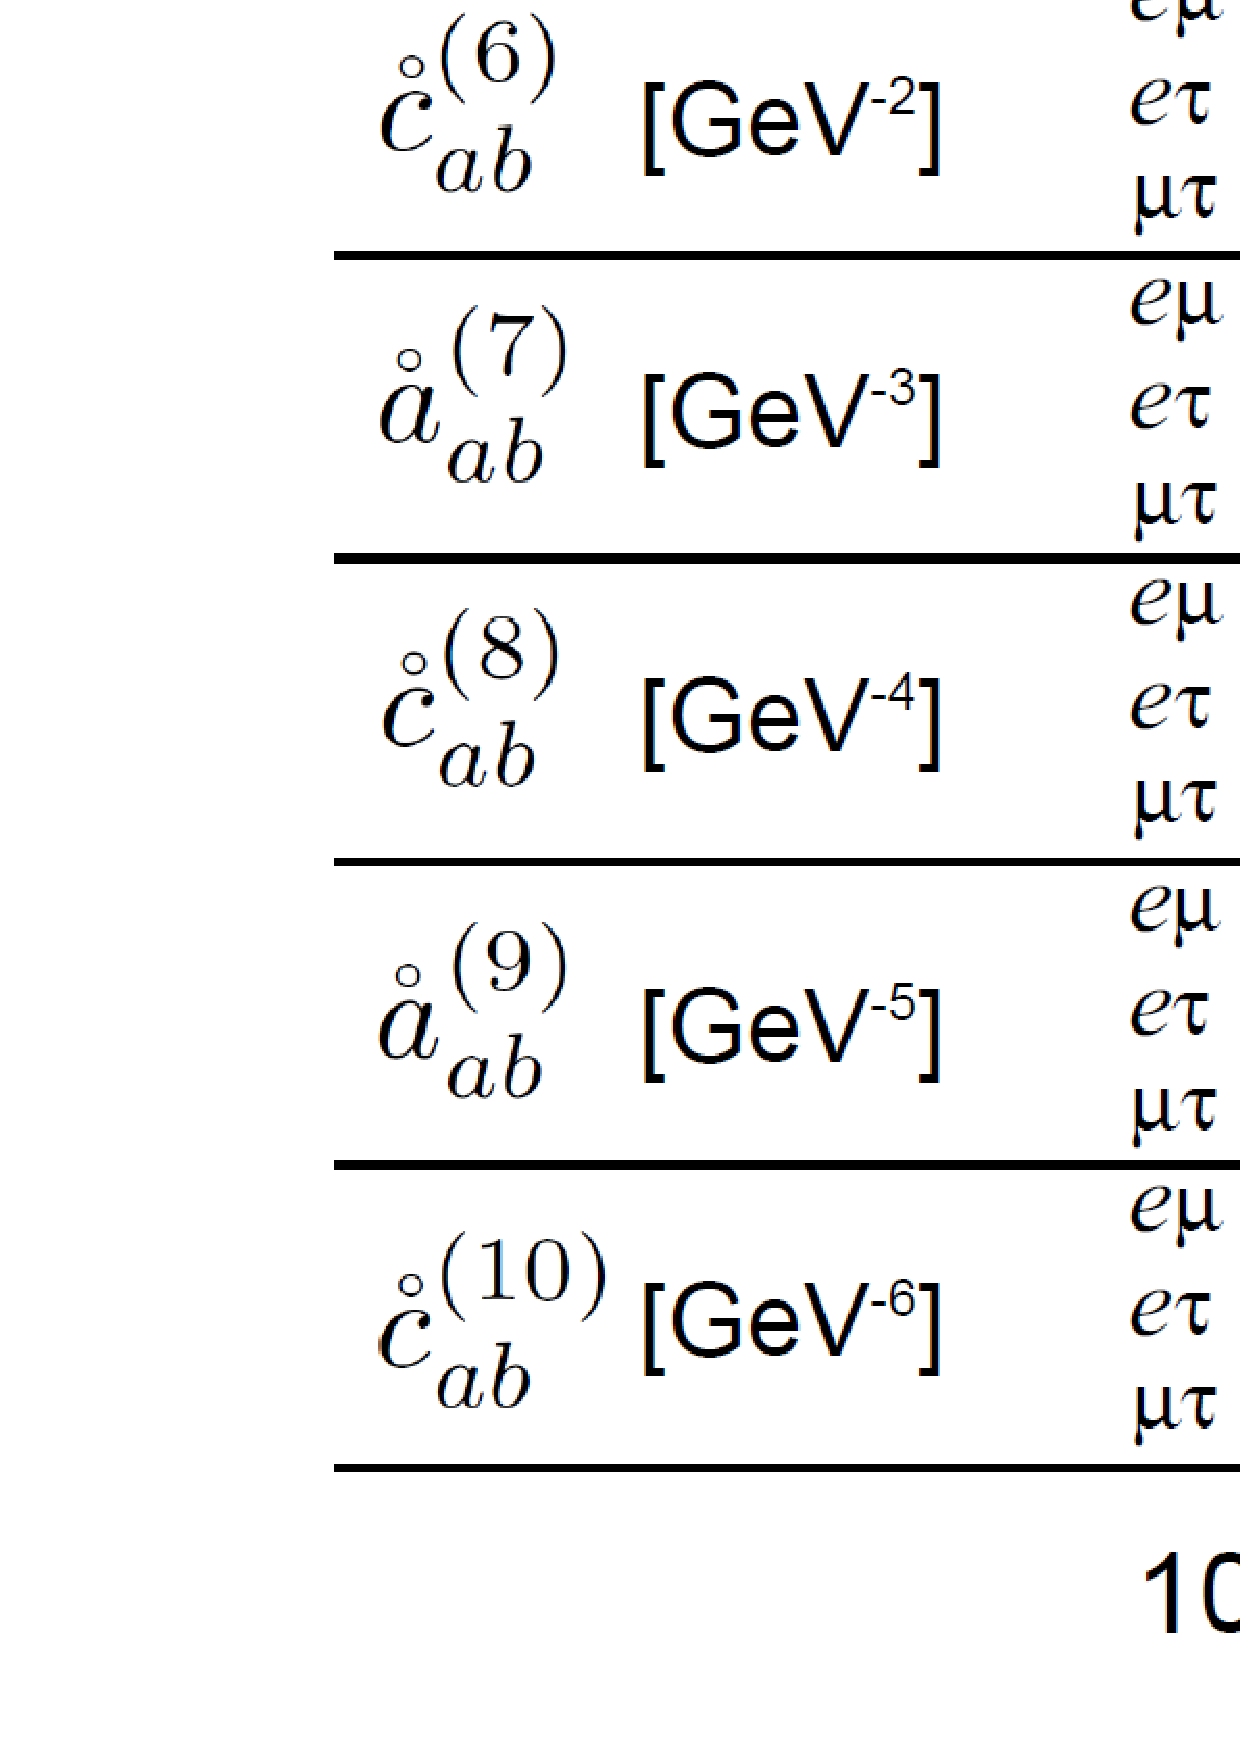
\includegraphics[width=0.8\textwidth]{DUNE-atm.pdf}
\end{dunefigure}

\begin{dunefigure}[Atmospheric fluxes of neutrinos and antineutrinos 
as a function of energy in the nonminimal isotropic SME]{fig:atm2}{Atmospheric fluxes of neutrinos and antineutrinos as a function of energy for convention oscillations (dashed line) and in the nonminimal isotropic SME (solid line).}
\includegraphics[width=0.8\textwidth]{DUNE-atm2.pdf}
\end{dunefigure}

%\begin{description}
%\item[Sensitivity:] Table describing NSI sensitivity (exists) . 
%\end{description}

\subsection{Reconstruction of atmospheric neutrinos}
\label{sec:nonaccel-atm-reco}

\begin{description}
\item[Sensitivity:] Results with latest reconstruction - flavor identification?  (early 2018) [I don't think we will have this.]
\end{description}
